\section[Main objective]{Main objective}
\label{sec:main_objective}

The \textbf{main object} of the project is to:

\begin{itemize}
\item Generate a reliable \textbf{time series forecast} based on sales from Favorita stores. 
\end{itemize}

Favorita stores is a  grocery retail store based in Ecuador. Producing an accurate forecast could lead to decreased food waste related to overstocking and improve customer satisfaction. All the code can be found in the following \href{https://github.com/razielar/forecasting_retail-store}{GitHub repository}, further information can be found in \nameref{sec:supp_info}.

\clearpage

\section[Data description]{Data description}
\label{sec:data_description}

The dataset comes from \textbf{Kaggle}, named: \href{https://www.kaggle.com/competitions/store-sales-time-series-forecasting/data}{Store Sales - Time Series Forecasting}. The Kaggle dataset contains sales data from \textit{Corporación Favorita}, a large Ecuadorian-based grocery retailer. Kaggle provides you with 7 diffeent files (see \autoref{tab:files} for more details). 

\begin{table}[!htb]
  \caption[Kaggle files description]{\textbf{Kaggle files description}. Files are alphabetically sorted.}
  \begin{scriptsize}
    \begin{tabulary}{0.65\linewidth}{ccl}
      \textbf{Number} & \textbf{File Name} & \textbf{Description} \\ \hline
      1 & holiday\_events.csv & Relevant holidays in Ecuador  \\
      2 & oil.csv & Oil prices from 2013 to 2017  \\
      3 & sample\_submission.csv & submission example  \\
      4 & stores.csv & Stores metadata  \\
      5 & test.csv & Stores and family products  \\
      6 & train.csv & Sales by store and product-family from 2013-01 to 2017-08  \\
      7 & transactions.csv & Number of transactions by store  \\
    \end{tabulary}
  \end{scriptsize}
  \label{tab:files}
\end{table}

The training data represents 99\% of the data, including dates from 2013-01-01 to 2017-08-16 (55.5 months), 54 stores placed in different cities within Ecuador, and 33 family-products (see \autoref{fig:store_summary}). The testing data includes dates from 2017-08-16 to 2017-08-31 (15 days).

\begin{figure}[!htb]
  \centering
  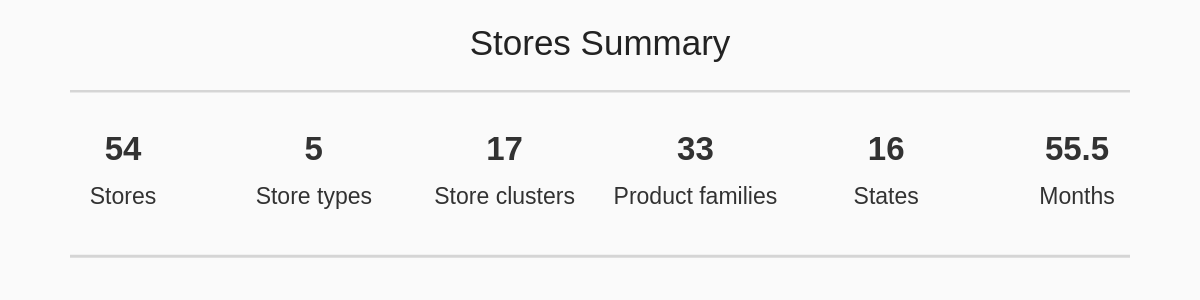
\includegraphics[width=0.9\textwidth]{plots/data_description/stores_summary.png}
  \caption[Summary of the training dataset]{\textbf{Summary of the training dataset}. The cluster information denotes similarity between stores.}
  \label{fig:store_summary}
\end{figure}

\section[Data exploration and data cleaning]{Data exploration and data cleaning}
\label{sec:eda}

Performing an exploratory data analysis (EDA) of the sales from the training dataset, we can observe that grocery I, beverages, and produce are the top 3 most consumed products (see \autoref{fig:eda}) . Additionally, store type A, and cluster 5 are the most frequent among their classification (\autoref{fig:eda}).

\begin{figure}[!htb]
  \centering
  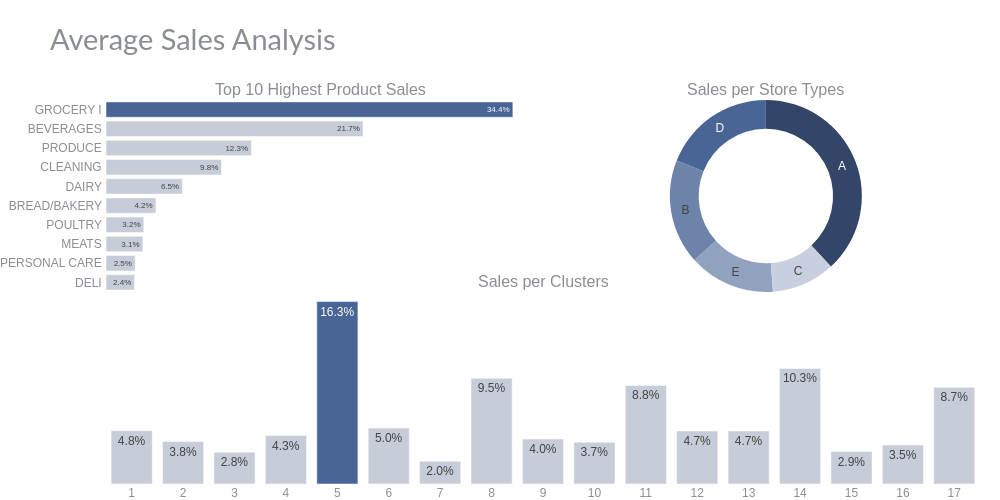
\includegraphics[width=0.9\textwidth]{plots/eda/sale_analysis.png}
  \caption[EDA of sales]{\textbf{EDA of sales}. The plot describes the sales by product, store type, and per cluster (left, right, and below, respectively). Darker blue represents higher sales. }
  \label{fig:eda}
\end{figure}


The sales represented by \autoref{fig:target} shows low-peaks at the end of each year, which is explained because the stores are closed at New years. Moreover, we can observe a pattern at each year, with increased sales at the end of the year which overlaps with the Christmas eves, suggesting a seasonal pattern. These patterns are highlighted after smoothing the sales data  with a 7 days moving average (the continuous red lines from the \autoref{fig:target}).

\begin{figure}[!htb]
  \centering
  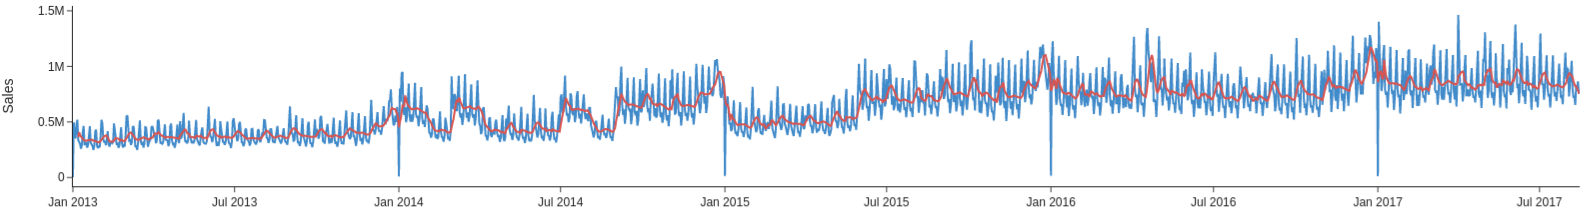
\includegraphics[width=0.9\textwidth]{plots/eda/target-time-series-plot-DF-testProc.png}
  \caption[Target time series data]{\textbf{Target time series data}. The y-axis represents the training sales from 2013-01-01 to 2017-08-15, and the x-axis shows the time in days (1087 days). The sales were aggregated by all stores and products (see \autoref{fig:store_summary}). The raw data, and smoothed data (7 days moving average) are denoted by the continuous blue, and red lines, respectively.}
  \label{fig:target}
\end{figure}

\subsection[Time series Decomposition]{Time series Decomposition}
\label{sec:decomposition}

Time series are defined as a sequence of data organized in time order. The key components of time-series are: trend, seasonality, and residuals, displayed in \autoref{fig:ts-decomposition}B, \autoref{fig:ts-decomposition}C, and \autoref{fig:ts-decomposition}D, respectively. Trend is the long-term direction of the time series, seasonality describes the periodic behavior such as holidays, and residuals represent the irregular fluctuations that we are not able to predict using the trend and/or seasonality.\autocite{moroff2021machine} 

In our target time series, we observe an upward trend, with a clear seasonality factor (this will be further analyzed below), and the residuals do not follow a random pattern. These insights will be used to select an adequate forecast model. 

\begin{figure}[!htb]
  \centering
  
\includegraphics[width=0.95\textwidth]{plots/eda/timseries_decomposition.png}
  \caption[Time series decomposition]{\textbf{Time series decomposition}. \textbf{(A)} Raw sales time series (sames as \autoref{fig:target}). \textbf{(B)} Trend of sales. \textbf{(C)} Seasonality of sales. \textbf{(D)} Residuals of sales. }
  \label{fig:ts-decomposition}
\end{figure}

\subsection[Stationarity and seasonality analyses]{Stationarity and seasonality analyses}
\label{sec:st_s_analysis}

The stationary and seasonality are relevant components to select the adequate machine learning model (such as ARIMA, SARIMA, etc.) to generate a reliable forecast. A stationary time series is defined, if their statistical properties such as mean, and variance are all constant, and independent of time.\autocite{moroff2021machine,feizabadi2022machine} In consequence, we implemented the \textit{Dickey-Fuller test} to assess stationarity. We obtained a \textit{p-value} of 0.09, using a significance level of 0.05, we can reject the null hypothesis (the series is stationary) concluding that our series is non-stationarity.


\begin{figure}[!htb]
  \centering
  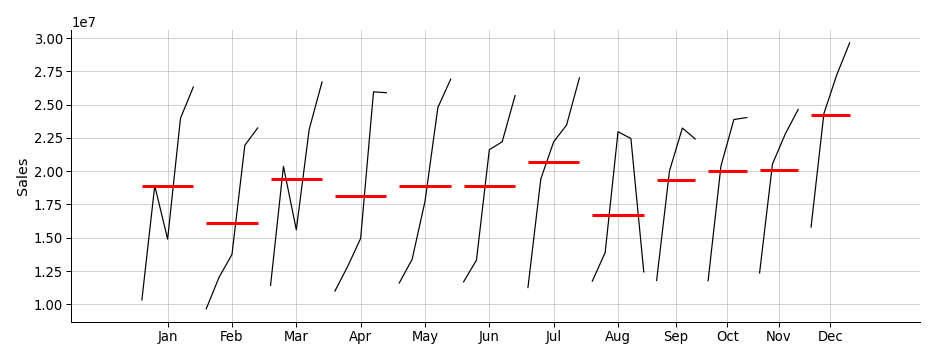
\includegraphics[width=0.7\textwidth]{plots/eda/seasonal_analysis.png}
  \caption[Analysis of seasonality]{\textbf{Analysis of seasonality}. The y-axis represents the sales aggregated by month, x-axis shows the analyzed months (from January to December), the horizontal red lines denote the sales average by month (55.5 months).}
  \label{fig:seasonal_plot}
\end{figure}

In terms of seasonality, we aggregate the sales for each month and we can clearly see on average an increase of sales during December (\autoref{fig:seasonal_plot}), which makes sense because Christmas and New years represent a season of the year with more transactions in other retail businesses. Furthermore, we highlighted February as the lowest sales month (\autoref{fig:seasonal_plot}). 

\begin{figure}[!htb]
  \centering
  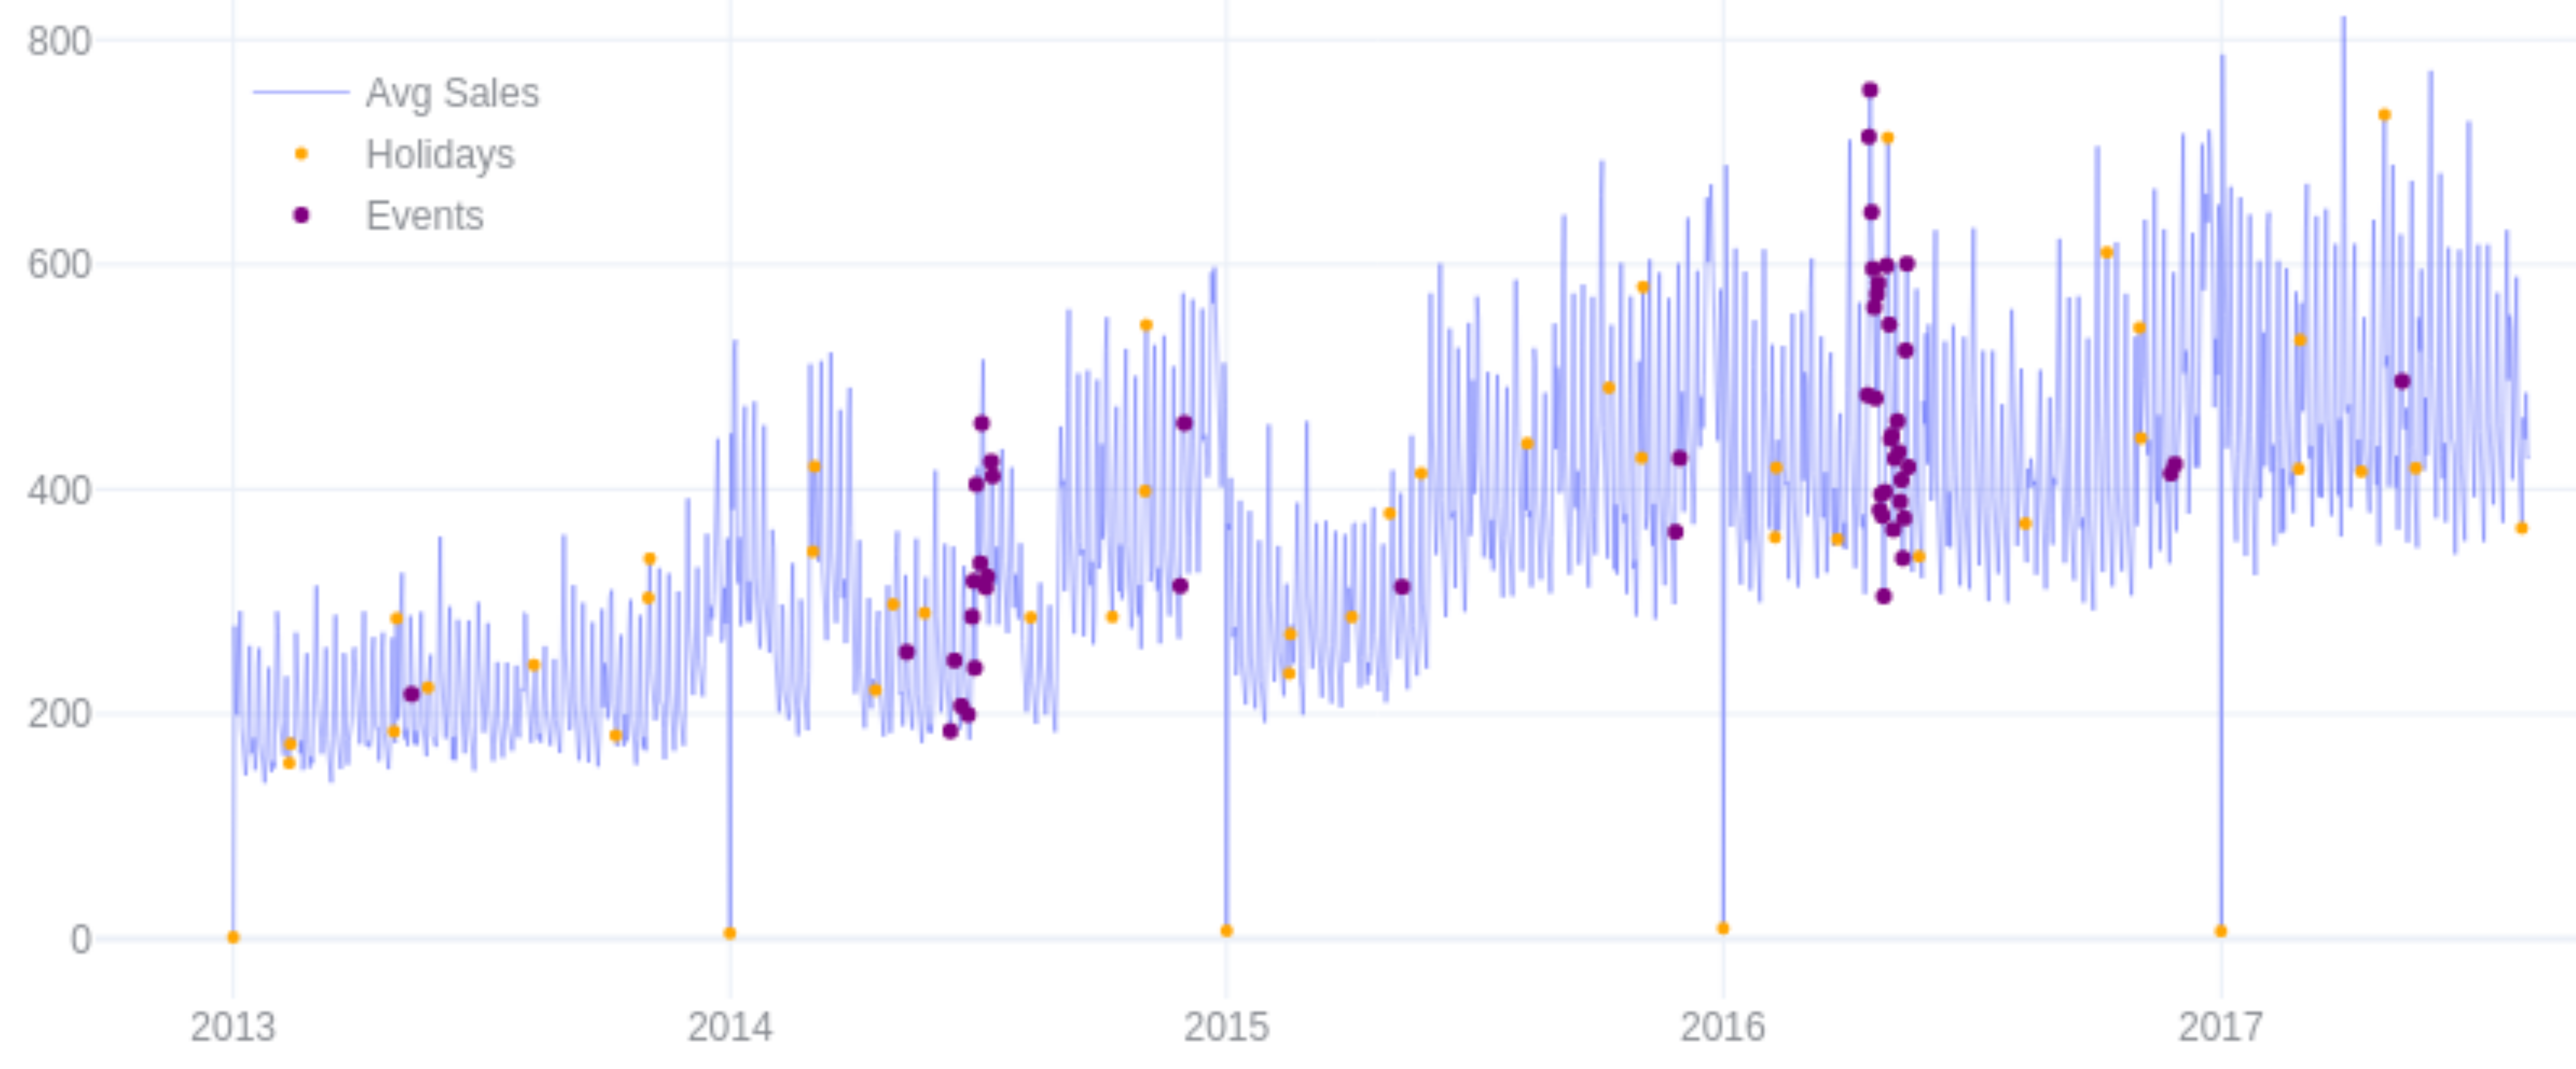
\includegraphics[width=0.6\textwidth]{plots/eda/holidayeffects.png}
  \caption[Holidays effect]{\textbf{Holidays effect}. Holidays and special events are represented as yellow, and purple dots, respectively.}
  \label{fig:holidays}
\end{figure}

Holidays are one of the most important factors for seasonality, and the Kaggle dataset provided us with relevant holidays and special events in Ecuador (see \autoref{tab:files}). Thus, we analyzed the effects of holidays on sales (see \autoref{fig:holidays}). We observed a reasonable correlation between holidays and sales. Consequently, holidays must be incorporated on the forecast.  

\clearpage

\section[Time series Models]{Time series Models}
\label{sec:forecast}

The main goal of the project is to generate a reliable forecast using the sales data from Favorita stores. After the EDA, we concluded that our data is not stationarity, possesses a strong seasonal effect, and holidays is a factor that should be considered in the forecast.  Therefore, the following models could be implemented:

\begin{itemize}
\item \textbf{SARIMAX}\autocite{hyndman2002state}: \underline{S}easonal \underline{ARIMA} using e\underline{X}ogenous data. Further, ARIMA stands for \underline{A}uto-\underline{R}egressive (p: dependence on past values), \underline{I}ntegrated (d: differencing) \underline{M}oving \underline{A}verage (q: dependence on past forecast errors). 
\item \textbf{LSTM}\autocite{hochreiter1997long}: \underline{L}ong-\underline{S}hort \underline{T}erm \underline{M}emory.
\item \textbf{GRU}\autocite{cho2014learning}: \underline{G}ated \underline{R}ecurrent \underline{U}nit.
\item \textbf{Facebook Prophet}\autocite{taylor2018forecasting}: is a forecasting procedure similar to a generalized additive model\autocite{hastie1987generalized} (GAM) where non-linear trends are fit with yearly, weekly, and daily seasonality, plus holiday effects.
\item \textbf{NeuralProphet}\autocite{triebe2021neuralprophet}: is a hybrid forecasting framework based on PyTorch and trained with standard deep learning methods.
\item \textbf{LightGBM}\autocite{ke2017lightgbm} (or other extreme gradient boosted method, \textit{e.g.} XGBoost): \underline{Light} \underline{G}radient-\underline{B}oosting \underline{M}achine.
\end{itemize}


Ideally, we would like to implement all of the  machine learning models mentioned above, do a benchmark taking into account: performance, computational-resources, training-time, and model-explainability; and compare their results. Nonetheless, due to time-constraints restrictions, we selected \textbf{Facebook Prophet} as our unique machine learning model to forecast the sales from Favorita stores. The reasons to select Facebook Prophet include:

\begin{enumerate}
\item A simple and flexible model (see \autoref{eq:prophet_eq} and  \autoref{eq:final_model}) that takes into account multiple human scale seasonality, and holidays that occur at irregular intervals.
\item Short training time (using the \textit{L-BFGS}  optimization algorithm\autocite{byrd1995limited}).
\item Low computation-resource demands and a Python module to easily implement the model (under the hood uses Stan\autocite{carpenter2017stan}).
\item Model explainability.
\item Previous experience with the model.
\end{enumerate} 

\subsection[Prophet as our Forecast model]{Prophet as our Forecast model}
\label{sec:forecast_model}

According to Taylor \textit{et al.}\autocite{taylor2018forecasting}, Facebook Prophet or Prophet (we are going to use Prophet from now on)  works best with time series that have strong seasonal effects (which is our case see \autoref{fig:ts-decomposition}C, and \autoref{fig:seasonal_plot}), holidays effect (\autoref{fig:holidays}), and typically handles outliers well. The model contains three main components: \textbf{1)} trend, \textbf{2)} seasonality, and \textbf{3)} holidays, which are combined in \autoref{eq:prophet_eq}:

\begin{align}\label{eq:prophet_eq}
y(t)= g(t) + s(t) + h(t) + \varepsilon_t  
\end{align}

Where $g(t)$ is the \underline{trend} function which models non-periodic changes in the value of the time series, $s(t)$ represents \underline{seasonality} (\textit{e.g.,} weekly and yearly seasonality), and $h(t)$ represents the effects of \underline{holidays} which occur on potentially irregular schedules over one or more days. The error term $\varepsilon_t$ represents changes not explained by the model; default prior $\varepsilon \sim N(0,0.5)$.

Prophets implements two types of trend models (logistic and linear trend model). In our project, the linear trend with changepoints was used, and can be written as \autoref{eq:trend_eq}. Where $\kappa$ stands for the growth rate, $\delta$ has the rate adjustments, $m$ is the offset parameter, and $\gamma_j$ is set to $-s_j\delta_j$ to make the function continuous. Additionally, prior $\delta_j \sim Laplace(0,\tau)$  where $\tau$ regularizes the trend flexibility.  

\begin{align}\label{eq:trend_eq}
g(t)= (\kappa + a(t)^T\delta)t + (m + a(t)^T\gamma)
\end{align}  

Next, seasonality $s(t)$ is modeled based on the Fourier series \autoref{eq:seasonal_eq}. Where $P$ represents the regular period we expect the time series to have (\textit{e.g.} $P=365.25$ and $P=7$ for yearly and weekly data, respectively). The term $X(t)\beta$ can be further explained with $X(t)$ and $\beta$ specified as vectors, see \autoref{eq:seasonal_ext} and \autoref{eq:seasonal_beta}. The term $N$ represents the order of the Fourier series. For yearly and weekly seasonality, the authors have found $N = 10$ and $N = 3$ to work well for most series problems, respectively. According to Taylor \textit{et al.}, prior $\beta \sim N(0,\sigma^2)$ where $\sigma$ regularizes the strength of seasonality.

\begin{align}\label{eq:seasonal_eq}
s(t) = \sum_{n=1}^N \left( a_n cos\left(\frac{2\pi nt}{P}\right) + b_n sin\left( \frac{2\pi nt}{P}  \right)  \right) = X(t)\beta
\end{align}

\begin{align}\label{eq:seasonal_ext}
X(t) = \left[ cos\left(\frac{2\pi1t}{P} \right), sin\left(\frac{2\pi1t}{P}\right),..cos\left(\frac{2\pi Nt}{P} \right), sin\left(\frac{2\pi Nt}{P}\right)  \right]
\end{align}

\begin{align}\label{eq:seasonal_beta}
\beta = [a_1,b_1,...a_N,b_N]
\end{align}

Subsequently, \autoref{eq:holiday_eq} represents the linear effects of holidays, and can be extended as \autoref{eq:holiday_2} which is a vector of dummies (1 indicates holiday and 0 otherwise), by assuming that the effects of holidays are independent. For each holiday $i$, let $D_i$ be the set of past and future dates for that holiday. And assign each holiday a parameter $\kappa_i$ which is the corresponding change in the forecast. As before, we use a prior $\kappa \sim N(0,\nu^2)$ where $\nu^2$ regularizes the holiday effects.

\begin{align}\label{eq:holiday_eq}
h(t)= Z(t)\kappa
\end{align}

\begin{align}\label{eq:holiday_2}
Z(t) = [1(t \in  D_1) ,..., 1(t \in  D_L)] 
\end{align}

Finally, combining all three models described above, we obtain the final model for our time series analysis that can be written as \autoref{eq:final_model}. Then, based on the five priors of the parameters and the data, we can find maximum a posterior (MAP) estimates for all parameters.

\begin{align}\label{eq:final_model}
y|m,\delta,\beta,\kappa,\varepsilon \sim N(g(t) + s(t) + h(t), \varepsilon)
\end{align}


\subsubsection[Prophet Hyperparameters]{Prophet Hyperparameters}
\label{sec:hyperparameters}

Prophet possesses 4 hyperparameters which can be tuned through cross validation, and are the following:

\begin{enumerate}
\item \textit{changepoint prior scale}: Determines the flexibility of the trend, in particular the trend changes, and the trend changepoints. If the value of changepoint prior scale is too small leads to underfit, if too large leads to overfit and in extreme scenarios leads with the trend capturing yearly seasonality. Further, higher values means more changepoints and more flexible trend.
\item \textit{seasonality prior scale}: Large values allow the seasonality to fit large fluctuations, and small values shrink the magnitude of the seasonality. The default value (see \autoref{tab:hyperparameters}) applies basically no regularization that is because the authors rarely see overfitting here.  
\item \textit{holidays prior scale}: This controls flexibility to fit holiday effects. Likewise to \textit{seasonality prior scale} the default value applies no regularization, since we usually have multiple holiday observations and can do a good job of estimating their effects. 
\item \textit{seasonality model}: This term, when possible, is best identified graphically by observing if the magnitude of seasonal fluctuations grows with the time series (multiplicative). Nonetheless, when it is not possible, it could be tuned. 
\end{enumerate}

\begin{table}[!htb]
  \caption[Prophet Hyperparameters]{\textbf{Prophet Hyperparameters}. The equation terms are defined above, see \nameref{sec:forecast_model}.}
  \begin{scriptsize}
    \begin{tabulary}{0.65\linewidth}{cccc}
      \textbf{Hyperparameter} & \textbf{Default} & \textbf{Recommended Range} & \textbf{Term} \\ \hline
      \textit{changepoint prior scale} & 0.05 & [0.001, 0.5] & $\tau$  \\
      \textit{seasonality prior scale} & 10  & [0.01, 10] & $\sigma$  \\
      \textit{holidays prior scale} & 10  & [0.01, 10] & $\nu$ \\
      \textit{seasonality model} & additive  & additive or multiplicative & $g(t) + s(t)$ or  $g(t) * s(t)$ \\
    \end{tabulary}
  \end{scriptsize}
  \label{tab:hyperparameters}
\end{table}

\subsubsection[Prophet Cross validation]{Prophet Cross validation}
\label{sec:cross-validation}

In our work, only the \textit{seasonality mode}  (either additive or multiplicative)  was tuned using cross validation (CV). CV in Prophet uses historical data and compares the forecasted values with the real values. There are three parameters we need to define:

\begin{enumerate}
\item \textit{initial}: the size of the initial training period. 
\item \textit{period}: space between two or more training periods, \textit{i.e.} cutoff dates. 
\item \textit{horizon}:  forecast horizon, \textit{i.e.} how many days/weeks,months,years are we going to make a forecast on. 
\end{enumerate}  

Since we have 1087 days we are using the initial 730 days (67.16\%) to predict the next 365 days, although all the results and plots presented show the performance metric (see \nameref{sec:error}) of a half year horizon. The period used was 180 days, leading to 4 forecasts with the following cutoffs: 2015-02-22, 2015-08-21, 2016-02-17, and 2016-08-15. \autoref{tab:cv} presents a more detailed description of the used parameters in the cross validation function.

\begin{table}[!htb]
  \caption[Cross validation in Prophet]{\textbf{Cross validation in Prophet}. The selected column displays the implemented parameters across all forecast results.}
  \begin{scriptsize}
    \begin{tabulary}{0.65\linewidth}{ccc}
      \textbf{Parameter} & \textbf{Default} & \textbf{Selected} \\ \hline
      \textit{initial} & 3*horizon & 730 days (67.16\%)  \\
      \textit{period} &  0.5*horizon: 182 days (2 cutoffs) & 180 days (4 cutoffs)   \\
      \textit{horizon} &   & 365 days  \\
    \end{tabulary}
  \end{scriptsize}
  \label{tab:cv}
\end{table}

\subsection[Performance Metric]{Performance Metric}
\label{sec:error}

To assess the performance of our models, we selected the mean absolute percentage error (MAPE) which is defined below:

\[ MAPE= \frac{100\%}{n} \sum_{t=1}^n \left| \frac{A_t - F_t}{A_t} \right|  \]

Where $A_t$ is the actual value (true value) and $F_t$ is the forecast result (predicted value). MAPE was selected as a performance metric because of its simplicity to represent the forecast errors within a percentage scale, where the lower the better. 

\clearpage

\section[Forecast Results]{Forecast Results}
\label{sec:results}

The sales data can be organized by store (54 stores) and by store and family product (1782 combinations). Therefore, as a starting point we aggregate all sales and generate 1 forecast (see \nameref{sec:general}). Then, generate a forecast by each store (54 forecasts; see \nameref{sec:forecast-store}). Finally, we generate a forecast of each product within each store (1782 forecasts; see \nameref{sec:forecast-product}).

\subsection[General Sales Forecast]{General Sales Forecast}
\label{sec:general}

\autoref{fig:general-forecast} shows the forecast outcome obtained aggregating all the sales, obtaining a MAPE of 22.26\%. 

\begin{figure}[!htb]
  \centering
  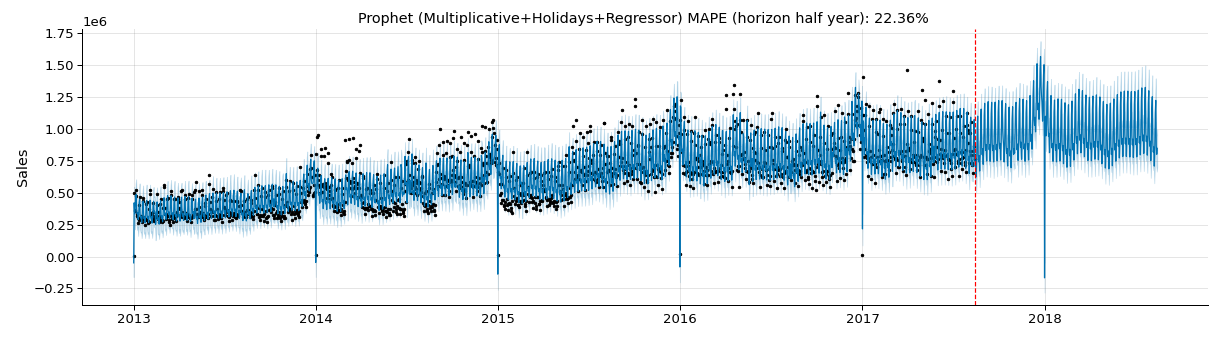
\includegraphics[width=0.9\textwidth]{plots/forecast/forecast_prophet.png}
  \caption[General Sales Forecast]{\textbf{General Sales Forecast}. Blue lines denotes the forecast, and black dots describe the actual values. Forecast is represented after the red dashed line. }
  \label{fig:general-forecast}
\end{figure}

After experimenting with different hyperparameters and conditions,  the Prophet model with the highest performance (the lowest MAPE) considers the following: 

\begin{enumerate}
\item A multiplicative seasonality mode.
\item Uses the provided holidays (holiday\_events.csv).
\item Custom regressor representing the store closing days.
\end{enumerate}


We observe a correct modeling of the training data, and correctly modeling the pronounced dips around Christmas and New Year (\autoref{fig:general-forecast}). Model explainability is an important factor to select a final model, in addition to performance, and computational training time. Prophet comes with an integrated explanation of the model components including the effects of holidays, weekly and yearly seasonality which helps to assess the performance of the forecast.

In consequence, the forecast components are displayed in \autoref{fig:forecast-components}. A sales increase is reported on the holiday component (\autoref{fig:forecast-components}A), which is expected in the retail business. In terms of weekly and yearly seasonality, Saturday and Sunday; and December are the periods with the highest sales, respectively (\autoref{fig:forecast-components}B and C).

\begin{figure}[!htb]
  \centering
  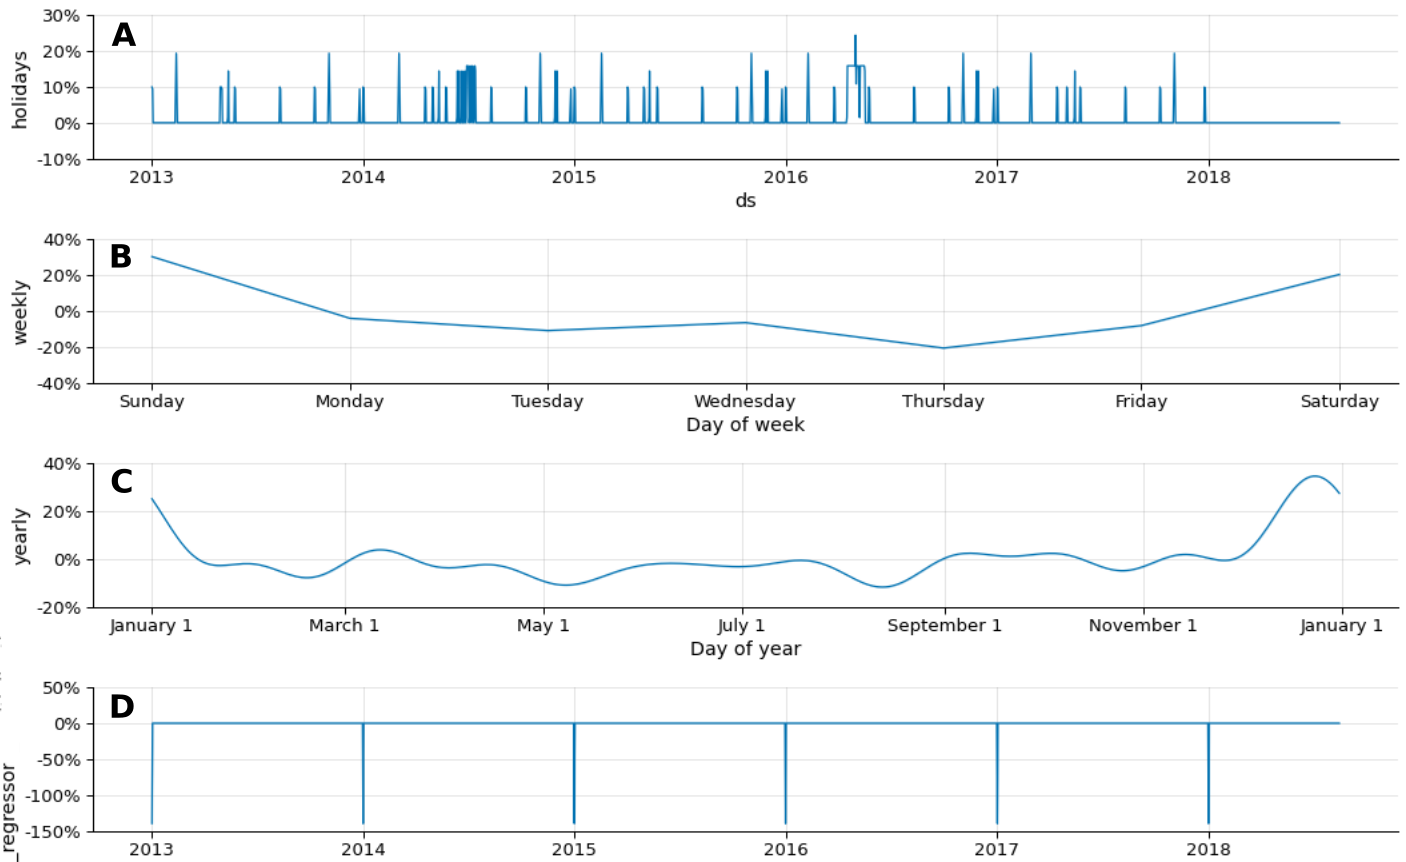
\includegraphics[width=0.7\textwidth]{plots/forecast/forecast_prophet-components.png}
  \caption[General Forecast Components]{\textbf{General Forecast Components}. The components of the final Prophet model, which considers a multiplicative seasonality, holidays, and a custom regressor represented on \autoref{fig:general-forecast}. \textbf{(A)} The holiday component. \textbf{(B)} Weekly seasonality. \textbf{(C)} Yearly seasonality. \textbf{(D)} Regressor considering the store closing days.}
  \label{fig:forecast-components}
\end{figure}

The regressor displays the store closing days which explains the pronounced dips around Christmas and New Year (\autoref{fig:forecast-components}D). In conclusion, we can state that our proposed models possess a moderate error (MAPE of 22.26\%), and the forecast components are in alignment of what we would expect of the retail business.   

\subsection[Sales Forecast by Store]{Sales Forecast by Store}
\label{sec:forecast-store}

Our dataset contains 54 stores. Thus, one time series model was produced to each store leading to 54 different Prophet models. In this scenario, a vanilla Prophet model was fitted to each store. Obtaining a mean MAPE of 36.87\%, twelve random stores are represented by \autoref{fig:forecast-store}, where the orange lines show the sales forecast by store. For better figure representation, the stores are displayed from 2017-05 to 2017-09 to highlight the last dates. 

\begin{figure}[!htb]
  \centering
  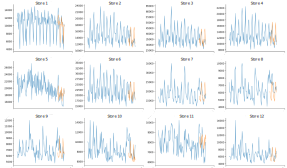
\includegraphics[width=0.9\textwidth]{plots/forecast/forecast_bystore.png}
  \caption[Forecast by Store]{\textbf{Forecast by Store}. The x-axis represents the dates from 2017-05 to 2017-09, the y-axis shows the sales for each store. The blue and orange lines display the store sales and forecast, respectively.}
  \label{fig:forecast-store}
\end{figure}

As expected, we obtained a higher error compared to the general sales forecast (36.87\% vs. 22.26\%). The reasons are: each store has a different sales pattern, and each Prophet model should be tuned for each store. In addition, a data normalization (such as $log$ transformation) could be implemented to achieve a lower MAPE. Nonetheless some store predictions are reasonable, for instance for stores: 1, 3, 6, and 10 (\autoref{fig:forecast-store}). In contrast, for stores: 7, 8, and 11 the forecasts can be considered as non-correct (\autoref{fig:forecast-store}).

Overall, 88\% of the forecasts can be considered as correct with a mean MAPE of 25.96\% (see all the forecast plots at the \href{https://github.com/razielar/forecasting_retail-store}{GitHub repository}). Considering the complexity of time series forecasting and the different sales patterns for each store, we can label our results as satisfactory. In order to have a higher confidence on our predictions a visual inspection should be used before relying on our forecast predictions.

\subsection[Sales Forecast by Store and Product]{Sales Forecast by Store and Product}
\label{sec:forecast-product}

In this scenario, one vanilla Prophet model was fitted for each product for each store producing a total of 1782 forecasts. As we can see on \autoref{fig:forecast-store-product}, each product for each store presents a completely different sales behavior leading to a more complex forecast problem. On average, we obtained a MAPE of 61.02\% (see \autoref{tab:mape-results}). Consequently, we are not able to suggest to rely on our predictions following this approach. 

\begin{figure}[!htb]
  \centering
  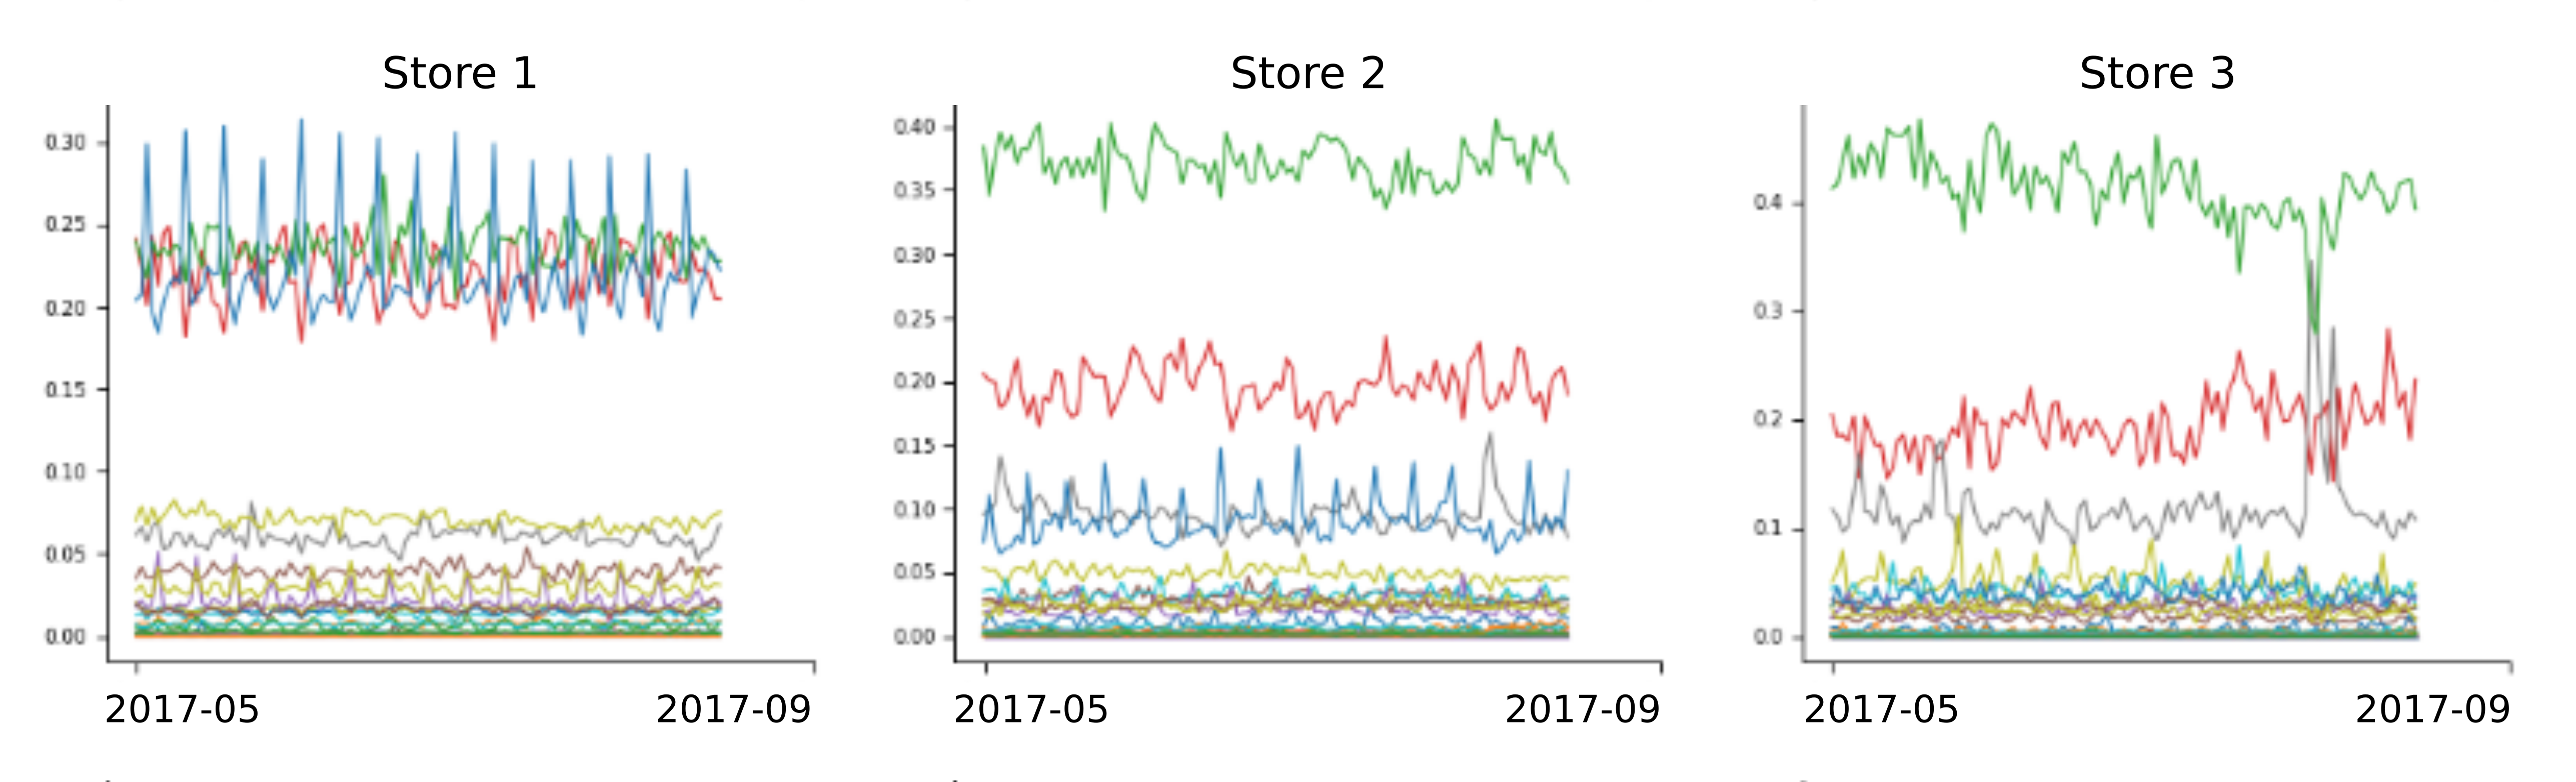
\includegraphics[width=0.9\textwidth]{plots/forecast/forecast_bystore_product.png}
  \caption[Forecast by Store and Product]{\textbf{Forecast by Store and Product}. The x-axis represents the dates from 2017-05 to 2017-09, the y-axis shows the sales for each store and product. The different color lines represent each sales product.}
  \label{fig:forecast-store-product}
\end{figure}

As \autoref{fig:forecast-store-product} shows each product type presents a different pattern on each store, explaining the low performance of our vanilla Prophet models, the same observation is maintained for all the 54 stores.

\begin{table}[!htb]
  \caption[Kaggle files description]{\textbf{Forecast Summary Results}. Results are sorted by MAPE.}
  \begin{scriptsize}
    \begin{tabulary}{0.65\linewidth}{ccc}
      \textbf{Forecast Approach} & \textbf{MAPE} & \textbf{Number of Predictions} \\ \hline
      General Sales Forecast & 22.26\% & 1  \\
      Sales Forecast by Store & 36.87\% & 54  \\
      Sales Forecast by Store and Product & 61.02\% & 1782  \\
    \end{tabulary}
  \end{scriptsize}
  \label{tab:mape-results}
\end{table}

In order to improve the predictions performance, we need to tune each model following the same approach of the \nameref{sec:general} (hyperparameter tuning, incorporating the holidays, etc.), but due to computational resources and time constraints these improvements were not implemented. Further improvements will be discussed in the \nameref{sec:next-steps} section. 

\section[Conclusions]{Conclusions}
\label{sec:conclusions}

\subsection[Recommendations]{Recommendations}
\label{sec:recommendations}

After performing general, store-specific, and product-specific forecasts we can recommend incorporating our general and store-specific forecast predictions, the latter after a visual inspection. Our general and store-specific predictions present a reasonable error, and their explainability components are in alignment of what we would expect of the retail business (see \autoref{fig:forecast-components} and \autoref{tab:mape-results}, respectively). 

Moreover, the training time of the models is not a constraint, and we could decrease the prediction horizon to decrease the MAPE metric, and retrain the models each month to avoid model drifting. Additional improvements in our general and store-specific will be discussed in the \nameref{sec:next-steps} section. Generating a reliable forecast for each product within each store could be a great interest for any retail business. Nevertheless, our results show on average a high error rate (see \autoref{tab:mape-results}) and we cannot recommend using our predictions following the product-specific approach. 

\subsection[Summary Key Findings]{Summary Key Findings}
\label{sec:key-findings}

\begin{enumerate}
\item Our target time series is nonstationary, with an upward trend, clear seasonality factor, and a reasonable correlation with holidays. 
\item Prophet model is suitable for our dataset, since it does have the types of features that Prophet is modeling such as a human seasonality, and holidays that occur at irregular intervals. Without seasonality and holiday effects, Prophet is just a piecewise linear regression.
\item We generated a reliable forecast (MAPE of 22.26\%) for general sales implementing a Prophet model with a multiplicative seasonality mode, using the provided holidays, and a custom regressor representing the store closing days. Moreover, the general forecast components are in agreement of what we would expect of the retail business. 
\item Regarding the sales forecast by store, we reached a moderate result (MAPE of 36.87\%) fitting 54 vanilla Prophet models for each store. Overall, 88\% of the forecasts can be considered as correct with a mean MAPE of 25.96\%. Thus, to incorporate our sales predictions a visual inspection needs to be used.
\item Sales forecast by store and product fitting a vanilla Prophet model for each combination led to poor results (MAPE of 61.02\%) and our sales predictions can not be implemented for this specific scenario. 
\end{enumerate}

\subsection[Next Steps]{Next Steps}
\label{sec:next-steps}

\begin{enumerate}
\item The Kaggle dataset includes the oil prices from 2013 to 2017 (see \autoref{tab:files}), which have a correlation with the store sales, and in general within the Ecuadorian economy. Due to data-constraints restrictions for the oil price for 2018  (365 day horizon), this additional information was not included in the analysis. However,  it should be included to improve the forecast performance. 
\item As mentioned above, the sales forecast by store and product obtained a non reliable outcome. Nonetheless, this can be tackled by tuning each model to each time series leveraging  Apache Spark\autocite{spark2018apache} large-scale data processing (PySpark UDF: user defined function) , and Prophet hyperparameter to improve the predictions results. There are plenty of resources following this approach, such as  medium posts (\href{https://higee.io/parallel-model-training-with-prophet-and-spark-5f40be750f97}{Gee post}) , and GitHub repositories (\href{https://github.com/srivatsan88/End-to-End-Time-Series/blob/master/Multiple_Time_Series_using_Apache_Spark_and_Prophet.ipynb}{Avatar Srivatsan Srinivasan repository}).
\item Perform a benchmark using different time series models, particularly lightGBM or LSTM, taking into account: performance, computational-resources, training-time, and model-explainability. Next select the most suitable model or models for each time series.
\item Hierarchical time series is a very promising approach to assess.   
\end{enumerate}
